\documentclass[12pt]{article}

%\usepackage{mathptm}  
\usepackage{a4}
\usepackage{hyperref}
\usepackage{color}
\usepackage{graphicx}
\usepackage{fancyhdr}
\usepackage{multicol}
\usepackage{amstext}
\usepackage{amsmath}
%\usepackage{fullpage}
%\usepackage{parskip}
\usepackage[colon]{natbib}
%\usepackage{rotating}
\usepackage{pdflscape}
\usepackage{longtable}
\usepackage{caption}
\usepackage{subcaption}
%\usepackage[nomarkers,figuresonly]{endfloat}
\usepackage{amsfonts}
\usepackage{pifont}
\usepackage{authblk}
\usepackage{epstopdf}
\usepackage{multirow}
\usepackage{amsfonts}

\textwidth 160mm
\textheight 235mm
\oddsidemargin 0mm
\topmargin -15mm
\baselineskip 13pt
\parskip 1pc
\parindent 0pc

\pagestyle{fancy}
\cfoot{\thepage}

\renewcommand{\headrulewidth}{0.2pt}
\renewcommand{\footrulewidth}{0.2pt}

\newcommand\Bo{\mbox{\textit{Bo}}}  % Bond number
\newcommand\Ca{\mbox{\textit{Ca}}} %Capillary number

\definecolor{darkred}{rgb}{0.80,0.00,0.05}
\definecolor{blue}{rgb}{0.00,0.00,0.95}
\definecolor{darkgreen}{rgb}{0.00,0.60,0.0}
\definecolor{gray}{rgb}{0.95,0.9,0.9}

\usepackage{listings}
\lstset{language=C++}
\lstset{backgroundcolor=\color{gray}}
\lstset{breaklines=true}
\lstset{basicstyle=\ttfamily\small}
\lstset{showstringspaces=false}
\lstset{keywordstyle=\color{blue}\bfseries}
\lstset{commentstyle=\ttfamily\small\color{darkgreen}}
\lstset{identifierstyle=\color{darkred}\bfseries}
\lstset{numbers=left,numberstyle=\tiny}
\lstset{columns=fixed,basewidth=0.45em}

\DeclareMathOperator\erf{erf}

\linespread{1.5}

\begin{document}
\thispagestyle{empty}

\title{Low Reynolds number gravitational settling of a sphere through a fluid-fluid interface: Modelling using a boundary integral method}

\author[1]{Paul Jarvis\footnote{Corresponding author:paul.jarvis@bristol.co.uk}}
\author[1]{Jon Blundy}
\author[1]{Katharine Cashman}
\author[1,2]{Herbert E Huppert}
\author[1]{Heidy Mader}
\affil[1]{\small School of Earth Sciences, University of Bristol, Wills Memorial Building, Queens Road, Bristol, BS8 1RJ, UK}
\affil[2]{\small Department of Applied Mathematics and Theoretical Physics, University of Cambridge, Wilberforce Road, Cambridge, CB3 0WA, UK}
\date{}
% NOTE: A full address must be provided: department, university/institution, town/city, zipcode/postcode, country.


\maketitle

\begin{abstract}


\end{abstract}


\section{Introduction}


\section{Theoretical Development}

The problem being modelled is the low Reynolds number gravitational settling of a sphere towards an initialy horizontal interface separating two density stratified, immiscible, semi-infinte fluids (figure~\ref{fig:params}). The fluids are characterised by the velocity $\mathbf{u}_{l}(\mathbf{x})$ and pressure $p_{l}(\mathbf{x})$ fields where $l = 1,2$ denotes the fluid and $\mathbf{x}$ is a position vector. The dynamic pressure is defined as

\begin{equation}
\label{equ:dyn_p}
p_{\text{d},l}(\mathbf{x}) = p_{l}(\mathbf{x}) - \rho_{l} \mathbf{g} \cdot \mathbf{x} ,
\end{equation}

where $\mathbf{g}$ is acceleration due to gravity. This allows the stress tensor to be defined as

\begin{equation}
\label{equ:stress}

\end{equation}

  \begin{figure}
    $$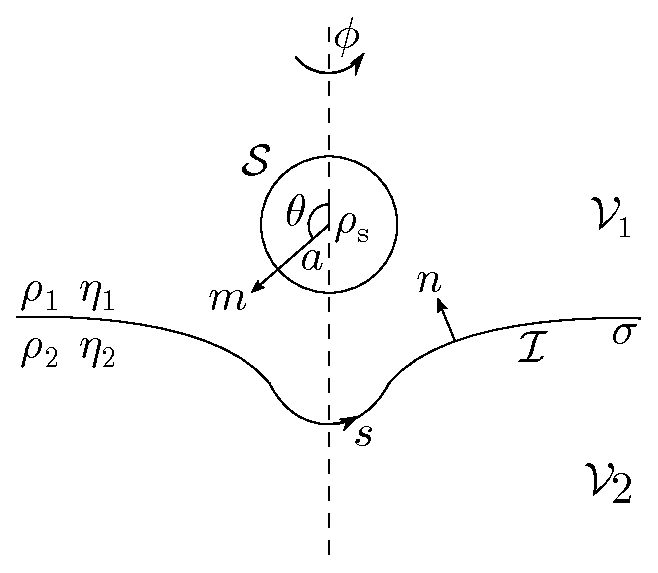
\includegraphics[width=0.8\textwidth]{formulation.eps}$$
    \caption{Diagrammatic representation of the system. A sphere falls under gravity, at low Reynolds number, towards an initially horizontal interface between two density stratified, immiscible semi-infinite fluids. See table~\ref{tab:symbols} for definition of symbols. \label{fig:params}}
  \end{figure}

    \begin{longtable}{|c|c|}
    \caption{Definition of symbols. \label{tab:symbols}} \\ % title name of the table
    \hline
    Symbol & Definition \\  
    \hline % inserts single-line
    $a$                                                    & Sphere radius           \\
    $\mathbf{g} = (-9.81 \text{m s}^{-2}) \mathbf{\hat{z}}$ & Acceleration due to gravity \\      
    $\mathcal{I}$                                          & Surface of interface \\
    $l = 1,2$                                              & Fluid label \\
    $m$                                                    & Outward normal to sphere surface \\
    $n$                                                    & Normal to interface (points into fluid 1) \\
    $p_{l}(\mathbf{x})$                                     & Pressure field of fluid $l$ \\
    $p_{\text{d},l}(\mathbf{x}) $                             & Dynamic pressure of fluid $l$ \\
    $s$                                                    & Arc length along interface measured from axis \\
    $\mathcal{S}$                                          & Surface of sphere \\
    $\mathbf{u}_{l}(\mathbf{x})$                            & Velocity field of fluid $l$ \\
    $\mathcal{V}_{l}$                                       & Volume of fluid $l$ \\
    $\mathbf{x}$                                           & Position vector \\
    $\mathbf{\hat{z}}$                                     & Unit vector in the upward vertical direction \\
    $\eta_{l}$                                              & Viscosity of fluid $l$ \\ 
    $\theta$                                               & Polar angle with respect to sphere centre \\
    $\rho_{l}$                                              & Density of fluid $l$   \\
    $\rho_{\text{s}}$                                         & Sphere density          \\
    $\sigma$                                               & Interfacial Tension     \\
    $\phi$                                                 & Azimuhtal angle with respect to axis of motion \\
    \hline % inserts single-line
  \end{longtable}


%\bibliographystyle{plainnat}

%\bibliography{fluids}


\end{document}